\documentclass{standalone}
\usepackage{tikz}

\begin{document}

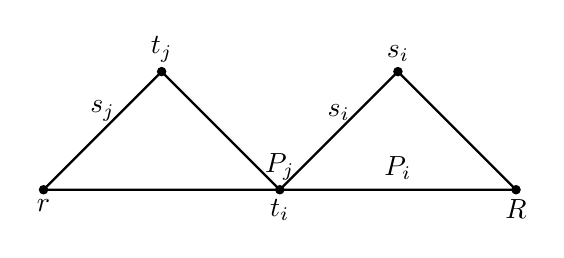
\begin{tikzpicture}[scale=1.5]
    % Define coordinates
    \coordinate (A) at (0,0);
    \coordinate (B) at (1,1);
    \coordinate (C) at (2,0);
    \coordinate (D) at (3,1);
    \coordinate (E) at (4,0);
    
    % Draw the main polygon
    \draw[thick] (A) -- (B) -- (C) -- (D) -- (E) -- cycle;
    
    % Draw dashed lines
    \draw[dashed] (A) -- (B) node[midway,above] {$s_j$};
    \draw[dashed] (C) -- (D) node[midway,above] {$s_i$};
    \draw[dashed] (E) -- (A) node[midway,above] {$P_j$};
    \draw[dashed] (E) -- (C) node[midway,above] {$P_i$};
    
    % Draw small circles at the vertices
    \filldraw (A) circle (1pt) node[below] {$r$};
    \filldraw (B) circle (1pt) node[above] {$t_j$};
    \filldraw (C) circle (1pt) node[below] {$t_i$};
    \filldraw (D) circle (1pt) node[above] {$s_i$};
    \filldraw (E) circle (1pt) node[below] {$R$};
\end{tikzpicture}

\end{document}